\documentclass[11pt]{article}

% Change "review" to "final" to generate the final (sometimes called camera-ready) version.
% Change to "preprint" to generate a non-anonymous version with page numbers.
\usepackage[review]{acl}

% Standard package includes
\usepackage{times}
\usepackage{latexsym}
\usepackage{booktabs}
\usepackage{amsmath}
\usepackage{amssymb}
\usepackage{array}
\usepackage{multirow}
% For proper rendering and hyphenation of words containing Latin characters (including in bib files)
\usepackage[T1]{fontenc}
% For Vietnamese characters
% \usepackage[T5]{fontenc}
% See https://www.latex-project.org/help/documentation/encguide.pdf for other character sets

% This assumes your files are encoded as UTF8
\usepackage[utf8]{inputenc}

% This is not strictly necessary, and may be commented out,
% but it will improve the layout of the manuscript,
% and will typically save some space.
\usepackage{microtype}

% This is also not strictly necessary, and may be commented out.
% However, it will improve the aesthetics of text in
% the typewriter font.
\usepackage{inconsolata}

%Including images in your LaTeX document requires adding
%additional package(s)
\usepackage{graphicx}
\usepackage{float} % Bổ sung gói float để sử dụng tham số [H]

% Give TeX a little extra flexibility in the narrow two-column measure.
\setlength{\emergencystretch}{1.5em}
\hbadness=10000

% If the title and author information does not fit in the area allocated, uncomment the following
%
%\setlength\titlebox{<dim>}
%
% and set <dim> to something 5cm or larger.

\title{Dynamic Geometric Regularization with Optimal Transport for Zero-Shot Cross-Lingual Question Answering}

% Author information can be set in various styles:
\author{First Author \\
  URA Research Group, Ho Chi Minh City University of Technology (HCMUT), Vietnam National University Ho Chi Minh City (VNU-HCM), Vietnam \\
  Ho Chi Minh city, Vietnam \\
  \texttt{vinh.vo1205@hcmut.edu.vn} \\\And
  Second Author \\
  Affiliation / Address line 1 \\
  Affiliation / Address line 2 \\
  Affiliation / Address line 3 \\
  \texttt{email@domain} \\}

\begin{document}
\maketitle
\begin{abstract}

Zero-shot cross-lingual extractive question answering (XQA) aims to transfer reasoning ability from high-resource languages to low-resource languages without relying on machine translation. Existing alignment-based approaches often suffer from over-alignment, where aggressive representation matching improves cross-lingual transfer but weakens source-language discriminability and answer boundary localization. To address this issue, we propose a curriculum-guided Optimal Transport framework that jointly regularizes representation alignment across spatial, domain, and temporal dimensions. Our approach employs a teacher--student architecture with frozen teacher representations, Optimal Transport alignment, anchor regularization for preserving source-language knowledge, and a curriculum margin scheduling strategy that gradually relaxes alignment constraints during training to maintain discriminative QA boundaries. Unlike methods that require additional trainable alignment modules, our framework operates directly on pretrained multilingual representations with minimal architectural overhead. Experiments on XQuAD and MLQA demonstrate consistent improvements in Vietnamese zero-shot transfer while maintaining competitive English performance. Extensive ablation studies further show that curriculum margin scheduling effectively balances cross-lingual adaptation and source-language retention, leading to a more stable and robust optimization process.

\end{abstract}

\section{Introduction}
Despite the remarkable success of multilingual pretrained language models, zero-shot cross-lingual extractive question answering (XQA) remains challenging, particularly for low-resource languages. Although models such as XLM-R encode multilingual knowledge within a shared semantic space, transferring answer localization ability from English to another language remains far from trivial.

Existing alignment methods frequently struggle to balance cross-lingual transfer performance with source-language retention. Current representation-level alignments, including standard contrastive learning and optimal transport, typically enforce symmetric objectives. Since both languages are simultaneously optimized toward a shared representation, the stronger English representation is also updated, gradually sacrificing source-language discriminability—a phenomenon often observed as catastrophic forgetting. Furthermore, these conventional methods tend to perform static alignment everywhere and all at once. We identify that this excessive, unregulated spatial pulling reduces inter-token discriminability, causing severe answer-boundary ambiguity. The fundamental failure mode lies in the conflation of two structurally distinct goals: semantic feature alignment and decision-boundary preservation.

To address this, we argue that alignment should not be a monolithic operation. Instead, it must be progressively coordinated across three complementary dimensions: space (geometry-aware spatial mapping), domain (source-language consistency), and time (temporal curriculum learning).

Building on this insight, we propose a Curriculum-Guided Geometry-Aware Optimal Transport framework. Rather than blindly forcing target representations into the source space, our framework dynamically decouples semantic alignment from decision-boundary preservation. At the core of our approach is a novel Curriculum Margin Preservation mechanism operating directly in the task (logit) space. By temporally scheduling margin constraints alongside asymmetric Optimal Transport at intermediate layers, the model learns to structurally align target-language concepts without collapsing the inter-token boundaries critical for precise span extraction.

Our main contributions are summarized as follows:
\begin{itemize}
    \item \textbf{Scientific Insight:} We identify that over-alignment in zero-shot cross-lingual QA stems from the inherent conflict between representation-level semantic mapping and token-level decision boundary preservation, which directly leads to answer-boundary ambiguity and source-language degradation.
    \item \textbf{Novel Methodology:} We propose a curriculum-guided Optimal Transport framework that coordinates cross-lingual transfer across space, domain, and time. This framework successfully decouples semantic alignment from boundary preservation through a novel temporal Curriculum Margin mechanism and an asymmetric Teacher-Student architecture.
    \item \textbf{Empirical Robustness:} Extensive experiments on MLQA and XQuAD demonstrate that our approach achieves superior zero-shot cross-lingual transfer to Vietnamese while largely preserving English source capabilities across both in-domain and held-out English benchmarks, significantly outperforming existing static alignment baselines.
\end{itemize}

\section{Related Work}

\subsection{Cross-Lingual Extractive QA}
The emergence of multilingual pre-trained language models, such as XLM-R, has significantly advanced zero-shot cross-lingual transfer \cite{conneau-etal-2020-unsupervised}. Early approaches primarily relied on translate-train or translate-test pipelines, which are fundamentally bottlenecked by external machine translation quality. Subsequent research established robust zero-shot evaluation benchmarks like XQuAD and MLQA to directly measure representation transferability without translationese artifacts \cite{artetxe-etal-2020-cross, lewis-etal-2020-mlqa}. 

Recent work has explored Cross-Lingual Knowledge Distillation (CLKD) to transfer reasoning ability from a high-resource teacher to a low-resource student \cite{gupta-etal-2023-cross}. To adapt these massive encoders efficiently, modern multilingual QA systems increasingly employ parameter-efficient fine-tuning techniques (e.g., LoRA) to acquire new language capabilities while maintaining pre-trained knowledge \cite{hu2021loralowrankadaptationlarge}. Despite their effectiveness, existing CLKD methods typically rely on symmetric alignment objectives. Consequently, when the source and target languages exhibit natural distributional disparities, rigidly forcing symmetric representation matching can distort the source language's established representational space, potentially inducing catastrophic forgetting.

\subsection{Representation Alignment}
Standard cross-lingual representation alignment often utilizes contrastive learning frameworks \cite{chi-etal-2021-infoxlm}. However, the underlying assumption of word-by-word isomorphism frequently breaks down when aligning morphologically diverse languages. Optimal Transport (OT), particularly via the entropy-regularized Sinkhorn distance, relaxes this constraint by framing alignment as a distribution matching problem \cite{cuturi2013sinkhorndistanceslightspeedcomputation}. In NLP, OT has been successfully applied to mitigate tokenization mismatches and align probabilistic latent variables \cite{sherborne-etal-2023-optimal}. However, when applied to token-level prediction tasks such as extractive QA, strong global alignment via OT may reduce local discriminability between candidate answer spans, causing answer-boundary ambiguity.

\subsection{Decision Boundaries and Margin-Based Curriculum}
Margin-based objectives have been instrumental in structuring representation spaces by explicitly modeling decision boundaries. This concept revolutionized computer vision through fixed-margin softmax variants (e.g., SphereFace\cite{wang2018cosfacelargemargincosine}, CosFace\cite{liu2018spherefacedeephypersphereembedding}, ArcFace \cite{Deng_2022}) that maximize inter-class variance. Recognizing that fixed margins struggle with ambiguous samples, subsequent frameworks introduced adaptive margins (e.g., AdaFace) to calibrate decision boundaries based on sample quality \cite{kim2023adafacequalityadaptivemargin}. Although margin-based learning has been widely explored for sequence-level tasks such as parallel corpus mining and retrieval \cite{artetxe-schwenk-2019-margin}, its application to preserving fine-grained token-level answer boundaries in cross-lingual extractive QA remains largely unexplored.

Parallel to boundary modeling, curriculum learning improves optimization by organizing training instances in a meaningful order of difficulty \cite{10.1145/1553374.1553380}. Existing cross-lingual curriculum methods primarily schedule training samples or task difficulty. In contrast, our work proposes scheduling the optimization geometry itself through a dynamically evolving margin, acting as a temporal curriculum that safely regulates the target language's convergence toward the source space.

\subsection{Research Gap}
Existing methods improve cross-lingual transfer by optimizing a single alignment objective. Some align representation spaces via OT, some preserve source knowledge via KD, and some optimize data via curriculum. However, these mechanisms have largely been investigated independently. We argue that effective cross-lingual transfer requires coordinated optimization across all three dimensions because they regulate complementary failure modes. As illustrated in Table \ref{tab:alignment_strategies}, spatial alignment improves semantic transfer, source preservation mitigates catastrophic forgetting, whereas the optimization curriculum prevents premature boundary collapse during training. 

\begin{table}[H]
\centering
\footnotesize
\setlength{\tabcolsep}{2pt}
\begin{tabular}{lccc}
\toprule
\textbf{Method} & \textbf{Spatial} & \textbf{Source} & \textbf{Opt.} \\
 & \textbf{Align.} & \textbf{Preservation} & \textbf{Curr.} \\
\midrule
Contrastive \cite{chi-etal-2021-infoxlm} & \checkmark & \texttimes & \texttimes \\
OT \cite{sherborne-etal-2023-optimal} & \checkmark & \texttimes & \texttimes \\
KD \cite{gupta-etal-2023-cross} & \texttimes & \checkmark & \texttimes \\
CL \cite{10.1145/1553374.1553380} & \texttimes & \texttimes & \checkmark \\
\midrule
\textbf{Ours} & \textbf{\checkmark} & \textbf{\checkmark} & \textbf{\checkmark} \\
\bottomrule
\end{tabular}
\caption{Comparison of cross-lingual adaptation strategies.}
\label{tab:alignment_strategies}
\end{table}

A natural question is why we decompose coordination into exactly three axes -- space, domain, and time -- rather than a finer or coarser partition. We argue this is not an arbitrary engineering choice but follows from the distinct level at which each axis operates: the spatial axis addresses a \emph{representation-level} problem (where target tokens sit relative to source tokens in the shared embedding space), the domain axis addresses a \emph{parameter-level} problem (how much the shared encoder is permitted to drift while adapting), and the temporal axis addresses an \emph{optimization-level} problem (the order and rate at which constraints are enforced during training). A failure at one level is not corrected by intervening at another: Table~\ref{tab:ablation_study} illustrates this empirically, as M2 (spatial alignment alone) actively degrades target-language transfer below the zero-shot baseline M0, showing that domain and temporal coordination are not incremental refinements on top of spatial alignment but address failure modes spatial alignment alone cannot reach. We do not claim this three-way split is the unique correct decomposition -- a finer-grained scheme could, for instance, separate the OT strength schedule from the margin schedule within the temporal axis -- but it is the coarsest partition at which each axis maps cleanly onto a previously-identified, distinct failure mode (over-alignment, catastrophic forgetting, and boundary collapse, respectively), which is why we adopt it as the natural granularity for this problem.

This observation motivates our coordinated alignment framework, which unifies spatial representation, source-language consistency, and temporal optimization into a single training paradigm.

% ==========================================
% SECTION 3: METHODOLOGY
% ==========================================

\section{Methodology}

\begin{figure*}[t]
    \centering
    
\includegraphics[width=0.95\textwidth]{figures/conceptual_diagram.png}
    \caption{Overview of our Coordinated Alignment Framework. Instead of relying on a monolithic alignment objective, we decouple the cross-lingual transfer process into three complementary dimensions: Spatial Alignment resolves the representation gap via Optimal Transport; Source Preservation mitigates catastrophic forgetting via a representation consistency anchor; and the Optimization Curriculum prevents decision-boundary collapse via dynamic margin scheduling.}
    \label{fig:conceptual_framework}
\end{figure*}

\subsection{Problem Formulation and Framework Overview}
To address the complementary failure modes of zero-shot cross-lingual transfer, we formulate the adaptation process as a coordinated optimization problem. Let $\mathcal{L}_{qa}$ denote the standard supervised question answering loss on the source language. We propose a framework that minimizes an overall objective decoupled into three regularization dimensions:
$$ \min_\theta \mathcal{L}_{total} = \lambda_{qa}\mathcal{L}_{qa} + \mathcal{L}_{space} + \mathcal{L}_{domain} + \mathcal{L}_{time} $$

We adopt a two-stage training paradigm utilizing a Teacher-Student architecture. In Stage 1, a teacher model is fine-tuned on the source language (English) to establish highly discriminative QA boundaries. In Stage 2, we freeze the teacher's weights and introduce a Low-Rank Adaptation (LoRA) student. 

Instead of relying solely on the final transformer layer for alignment—which heavily over-fits to task-specific predictive patterns—we apply a trainable softmax weighting across intermediate layers (specifically layers 6 through 9) to extract and aggregate language-agnostic semantic abstractions. We deliberately target these middle layers because probing analyses on transformer attention mechanisms have demonstrated that intermediate layers (e.g., layers 6 to 10) are particularly rich in capturing core structural and syntactic relations, such as dependency syntax and coreference \cite{clark-etal-2019-bert}. By structurally aggregating these deep relational representations, the student is then robustly optimized across the spatial, domain, and temporal dimensions.

\subsection{Spatial Coordination: Macro and Micro Alignment}
The spatial dimension ($\mathcal{L}_{space}$) aims to bridge the cross-lingual representation gap. We decompose this into macro-structural alignment via Optimal Transport ($\mathcal{L}_{ot}$) and micro-structural label projection via barycentric mapping ($\mathcal{L}_{span}$).

\textbf{Macro Alignment (OT):} Let $H^{src}$ and $H^{tgt}$ denote the normalized hidden representations of the source and target sequences at the intermediate layers. We define the transport cost matrix $C$ using the cosine distance:
$$ C_{ij} = 1 - \frac{h^{src}_i \cdot h^{tgt}_j}{\|h^{src}_i\| \|h^{tgt}_j\|} $$
We utilize the entropy-regularized Sinkhorn algorithm to find the optimal transport plan $T^*$. Crucially, we stop the gradient through the transport plan ($T^*.detach()$) so that the optimization only updates the representation geometry while treating the transport assignment as a fixed correspondence:
$$ \mathcal{L}_{ot} = \langle T^*.detach(), C \rangle_F $$

\textbf{Micro Alignment ($\gamma$-Barycentric Span Transfer):} Extractive QA requires precise token-level boundary detection. Standard cross-lingual distillation minimizes the divergence between source and target logits, but this fails when vocabulary dimensions mismatch or span positions shift across translations. To solve this, we leverage the learned transport plan $\gamma$ (equivalent to $T^*$) to structurally project the source model's predicted span distribution ($p^{src}$) into the target space, creating zero-shot pseudo-labels ($\tilde{p}^{tgt}$):
$$ \tilde{p}^{tgt}_{start} = \frac{\gamma^T p^{src}_{start}}{\sum_j \gamma_{\cdot j}} $$
The span-aware local alignment is then enforced via Kullback-Leibler divergence:
$$ \mathcal{L}_{span} = \frac{1}{2} \sum_{k \in \{start, end\}} D_{KL}(\tilde{p}^{tgt}_{k} \| p^{tgt}_{k}) $$
The total spatial coordination loss is defined as: $\mathcal{L}_{space} = \lambda_{ot}\mathcal{L}_{ot} + \lambda_{span}\mathcal{L}_{span}$.

\subsection{Domain Coordination: Source Preservation}
\label{sec:domain}
While spatial alignment successfully transfers semantic knowledge, updating shared parameters inherently risks corrupting well-established source language representations. To mitigate catastrophic forgetting, we coordinate the source domain ($\mathcal{L}_{domain}$).

Standard practices typically employ either strict parameter freezing (which heavily restricts cross-lingual adaptation capacity) or joint fine-tuning (which is computationally expensive and prone to gradient interference). Instead, we introduce a soft constraint mechanism. We minimize the $L_2$ distance between the token representations generated by the frozen English teacher ($h^{frz}_{src}$) and the actively adapting LoRA student ($h^{LoRA}_{src}$):
$$ \mathcal{L}_{domain} = \mathcal{L}_{reg} = \frac{1}{|\mathcal{V}|} \sum_{i \in \mathcal{V}} \| h^{LoRA}_{src,i} - h^{frz}_{src,i} \|^2_2 $$
This highly weighted regularization acts as a robust representation consistency anchor, ensuring the student network safely adapts to the target language without drifting from the source model's structural topology.

\subsection{Temporal Coordination: Margin Curriculum}
\label{sec:temporal}
The final dimension regulates optimization instability ($\mathcal{L}_{time}$). Pulling target representations towards the source space all at once frequently blurs the precise inter-token distinctions required for exact span extraction. To protect these boundaries, we enforce a margin constraint directly in the task decision boundary (logit space).

We define the source margin ($m_{src}$) as the confidence gap between the gold token logit and the hardest negative token logit, while the target margin ($m_{tgt}$) is the difference between its top-1 and top-2 logits:
$$ m_{src} = \text{logit}[s^{gold}] - \max_{j \neq gold} \text{logit}[j] $$
$$ m_{tgt} = \text{top1\_logit} - \text{top2\_logit} $$
$$ \mathcal{L}_{margin} = \text{ReLU}(m_{src}.detach() - m_{tgt}) $$

Imposing a rigidly large margin from the beginning forces premature optimization, exacerbating the geometric distortion, whereas a small margin causes negative transfer. To resolve this optimization conflict, we formulate the margin constraint as a temporal curriculum. By dynamically annealing the margin threshold across training epochs (e.g., scheduling the margin to decay from $1.0$ down to $0.3$), the model allows target-language representations to progressively align their semantic spaces before enforcing strict boundary discrimination. 
$$ \mathcal{L}_{time} = \lambda_{margin}\mathcal{L}_{margin} $$

\begin{figure}[H]
    \centering
    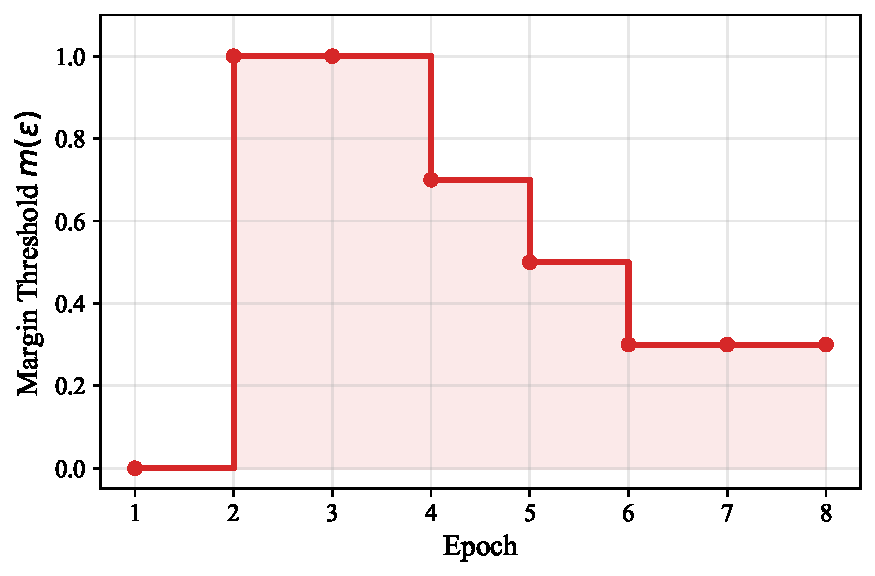
\includegraphics[width=0.85\linewidth]{figures/figure3b_margin_schedule.pdf}
    \caption{Curriculum margin schedule used during Stage-2 training: the task-space margin threshold $\lambda_{margin}$ is annealed in discrete steps from $1.0$ to $0.3$ across training epochs, progressively tightening the decision-boundary constraint as target-language representations converge.}
    \label{fig:margin_schedule}
\end{figure}

Figure~\ref{fig:margin_schedule} illustrates the concrete schedule used in our experiments.

\subsection{Overall Objective}
By integrating the aforementioned components, our coordinated alignment framework harmonizes spatial transfer, domain consistency, and temporal optimization into a unified training paradigm:
$$ \mathcal{L}_{total} = \lambda_{qa}\mathcal{L}_{qa} + \mathcal{L}_{space} + \mathcal{L}_{domain} + \mathcal{L}_{time} $$

\section{Experiments}

\subsection{Experimental Setup}
\label{sec:setup}
\textbf{Datasets and Evaluation:} We validate our coordinated alignment framework on extractive QA. In Stage 1, the teacher model is fine-tuned on the English SQuAD 2.0 dataset. For Stage 2 (student adaptation), we utilize a parallel loader containing English SQuAD 2.0 and the AIForge Vietnamese-SQuAD dataset. Crucially, the student receives no target-language ground truth labels during training, maintaining a strict zero-shot cross-lingual transfer paradigm. We evaluate the transfer performance on the Vietnamese splits of XQuAD \cite{artetxe-etal-2020-cross} and MLQA \cite{lewis-etal-2020-mlqa}. 

\textbf{Metrics:} We report the standard Exact Match (EM) and macro-averaged F1 scores. To explicitly measure the catastrophic forgetting of the source language, we introduce the Source Preservation Metric ($\Delta_{src}$), defined as the difference in English SQuAD 2.0 F1 scores before and after the Stage-2 student alignment ($\Delta_{src} = F1_{post-align} - F1_{pre-align}$). An optimal framework should maximize target-language EM/F1 while maintaining $\Delta_{src} \approx 0$.

\textbf{Implementation Details:} Our framework is built upon the XLM-RoBERTa backbone \cite{conneau-etal-2020-unsupervised}. For parameter-efficient training in Stage 2, we apply Low-Rank Adaptation (LoRA) \cite{hu2021loralowrankadaptationlarge} to the query, key, value, and dense projection matrices with rank $r=16$ and $\alpha=32$. The dynamic margin schedule anneals the threshold in discrete temporal steps (from $1.0$ down to $0.3$) across the training epochs. 

\subsection{Main Results: Zero-Shot Cross-Lingual Transfer}

\begin{table}[H]
\centering
\small
\setlength{\tabcolsep}{4pt}
\begin{tabular}{lcccc}
\toprule
\multirow{2}{*}{\textbf{Model}} & \multicolumn{2}{c}{\textbf{XQuAD-vi}} & \multicolumn{2}{c}{\textbf{MLQA-vi}} \\
\cmidrule(lr){2-3} \cmidrule(lr){4-5}
 & \textbf{EM} & \textbf{F1} & \textbf{EM} & \textbf{F1} \\
\midrule
XLM-R Zero-shot & 46.22 & 63.64 & 46.05 & 67.21 \\
Vanilla KD & 45.55 & 69.31 & 41.34 & 64.42 \\
Static Alignment (OT) & 38.66 & 57.63 & 36.08 & 56.06 \\
\midrule
\textbf{Ours (Coordinated)} & \textbf{51.26} & \textbf{71.22} & \textbf{46} & \textbf{68.1} \\
\bottomrule
\end{tabular}
\caption{Zero-shot cross-lingual transfer results on Vietnamese XQuAD and MLQA. Our coordinated framework outperforms the zero-shot baseline and vanilla KD on both benchmarks, with a large margin on XQuAD-vi and a smaller but consistent gain on MLQA-vi.}
\label{tab:main_results}
\end{table}

Table \ref{tab:main_results} presents the zero-shot transfer performance on the Vietnamese MLQA and XQuAD benchmarks. Compared to the zero-shot baseline and vanilla knowledge distillation, our coordinated alignment framework demonstrates substantial improvements in both Exact Match and F1 scores. The performance gain validates the efficacy of decoupling spatial transport from boundary preservation. By utilizing the $\gamma$-barycentric span projection, the student model successfully infers accurate target-language answer boundaries without requiring explicit target-domain supervision.

\subsection{Source Preservation Analysis}
\begin{table*}[t]
\centering
\small
\resizebox{\textwidth}{!}{%
\begin{tabular}{lcccccccccc}
\toprule
\multirow{2}{*}{\textbf{Configuration}} & \multicolumn{3}{c}{\textbf{SQuAD-EN (in-domain)}} & \multicolumn{3}{c}{\textbf{XQuAD-en (held-out)}} & \multicolumn{3}{c}{\textbf{MLQA-en (held-out)}} \\
\cmidrule(lr){2-4} \cmidrule(lr){5-7} \cmidrule(lr){8-10}
 & \textbf{Pre F1} & \textbf{Post F1} & \textbf{$\Delta_{src}$} & \textbf{Pre F1} & \textbf{Post F1} & \textbf{$\Delta_{src}$} & \textbf{Pre F1} & \textbf{Post F1} & \textbf{$\Delta_{src}$} \\
\midrule
Teacher (Stage 1 only) & 72.84 & 72.84 & 0.0 & 75.7 & 75.7 & 0.0 & 79.8 & 79.8 & 0.0 \\
Student, OT only (no $\mathcal{L}_{reg}$) & 72.84 & 69.29 & -3.55 & 75.7 & 73.38 & -2.32 & 79.8 & 76.67 & -3.13 \\
\midrule
\textbf{Student, Ours (OT + $\mathcal{L}_{reg}$)} & \textbf{72.84} & \textbf{73.27} & \textbf{0.43} & 75.7 & 74.8 & -0.9 & 79.8 & 79.4 & -0.4 \\
\bottomrule
\end{tabular}
}
\caption{Analysis of source preservation ($\Delta_{src}$) on English SQuAD 2.0 (in-domain, i.e.\ the Stage-1 training distribution), alongside held-out English XQuAD-en and MLQA-en (the exact English counterparts of the XQuAD-vi/MLQA-vi transfer targets used elsewhere in this paper). $\Delta_{src} = F1_{post\text{-}align} - F1_{pre\text{-}align}$.}
\label{tab:source_preservation}
\end{table*}

A critical failure mode in cross-lingual adaptation is the degradation of source-language capabilities due to shared parameter updates. As illustrated in the source preservation analysis, frameworks employing global spatial alignment without domain constraints suffer from severe catastrophic forgetting, evidenced by a significant drop in English QA performance ($\Delta_{src} \ll 0$). 

By integrating the source consistency anchor ($\mathcal{L}_{reg}$), our domain coordination mechanism successfully restricts the LoRA parameters from unlearning English syntax. The student model maintains a $\Delta_{src}$ approximating zero, providing empirical evidence that target-language topological mapping can be achieved without paying a substantial alignment tax on the source language.

The held-out columns in Table~\ref{tab:source_preservation} reinforce this picture consistently across all three benchmarks. Removing $\mathcal{L}_{reg}$ produces a clear drop on every benchmark -- $\Delta_{src}=-3.55$ on SQuAD-EN, $-2.32$ on XQuAD-en, and $-3.13$ on MLQA-en -- while our full configuration keeps $\Delta_{src}$ close to zero throughout ($+0.43$, $-0.9$, and $-0.4$, respectively). The gap between the two configurations is $2$--$4$ F1 points on every benchmark, indicating that the source-consistency anchor's benefit is not an artifact of the in-domain SQuAD-EN distribution but holds under held-out evaluation as well.

\subsection{Ablation Study}

\begin{table*}[t]
\centering
\small
\resizebox{\textwidth}{!}{%
\begin{tabular}{lccccccc}
\toprule
\multirow{2}{*}{\textbf{Configuration}} & \multicolumn{3}{c}{\textbf{Coordination Components}} & \multicolumn{2}{c}{\textbf{MLQA-vi (Target)}} & \multicolumn{2}{c}{\textbf{SQuAD-EN (Source)}} \\
\cmidrule(lr){2-4} \cmidrule(lr){5-6} \cmidrule(lr){7-8}
 & \textbf{Global ($\mathcal{L}_{ot}$)} & \textbf{Local ($\mathcal{L}_{span}$)} & \textbf{Time ($m$)} & \textbf{EM} & \textbf{F1} & \textbf{EM} & \textbf{F1} \\
\midrule
M0: Zero-shot Baseline & $\times$ & $\times$ & $\times$ & 46.05 & 67.21 & 64.26 & 72.84 \\
M1: Vanilla KD & $\times$ & $\times$ & $\times$ & 41.34 & 64.42 & 65.65 & 73.93 \\
M2: Global Align Only & $\checkmark$ & $\times$ & $\times$ & 36.08 & 56.06 & 66.08 & 72.75 \\
M3: Global + Local & $\checkmark$ & $\checkmark$ & $\times$ & 44.35 & 65.33 & 64.58 & 73.09 \\
M4: Static Boundary & $\checkmark$ & $\checkmark$ & Static & 45.41 & 67.41 & 65.64 & 73.9 \\
\midrule
\textbf{M5: Ours (Full Coordinated)} & \textbf{$\checkmark$} & \textbf{$\checkmark$} & \textbf{Dynamic} & \textbf{46} & \textbf{68.1} & \textbf{64.84} & \textbf{73.27} \\
\bottomrule
\end{tabular}
}
\caption{Ablation study isolating the variables of the coordinated alignment framework. All configurations from M1 to M5 utilize domain consistency ($\mathcal{L}_{reg}$) to anchor the source representation. The progression demonstrates the cumulative synergy of spatial and temporal regularizations.}
\label{tab:ablation_study}
\end{table*}

\begin{figure}[H]
    \centering
    
\includegraphics[width=1.05\linewidth]{figures/figure4_vi.pdf}
    \caption{Radar comparison of final validation F1 across the three evaluation axes (SQuAD-EN source, XQuAD-VI target, MLQA-VI target) for each ablation configuration (M0--M5 in Table~\ref{tab:ablation_study}). A larger enclosed area reflects a better joint source--target trade-off rather than a single-axis win.}
    \label{fig:F1-ablation}
\end{figure}

\begin{figure}[H]
    \centering
    
\includegraphics[width=1.05\linewidth]{figures/figure4_EM.pdf}
    \caption{Radar comparison of final validation EM across the same three axes and configurations as Figure~\ref{fig:F1-ablation}.}
    \label{fig:EM-ablation}
\end{figure}

To isolate the contributions of the spatial and temporal coordination mechanisms, we conduct an extensive ablation study (Table \ref{tab:ablation_study}). Note that, as stated in the table caption, every configuration M1--M5 already retains the domain-consistency term ($\mathcal{L}_{reg}$); its individual contribution is instead isolated separately in Table \ref{tab:source_preservation}, where removing $\mathcal{L}_{reg}$ causes English F1 to drop by $-3.55$ points relative to the pre-alignment teacher, consistent with catastrophic forgetting.

Within Table \ref{tab:ablation_study}, removing spatial macro-alignment ($\mathcal{L}_{ot}$, configuration M2) drastically reduces the overall F1 transfer score relative to M1, confirming that aligning intermediate hidden spaces is a prerequisite for target-language comprehension -- notably, M2 also under-performs the zero-shot baseline M0 on the target side, showing that global OT alignment alone can actively hurt transfer if left unregulated. Adding the micro-alignment term (M3, $\mathcal{L}_{span}$) largely recovers this loss and improves Exact Match, verifying that span-aware local alignment is necessary to convert global transport into precise boundary localization. Introducing the margin-based temporal component (M4, M5) then yields further, consistent gains on both EM and F1 on the target side, while source-side performance (SQuAD-EN) stays within a narrow band across all configurations (72.75--73.93 F1), since $\mathcal{L}_{reg}$ is active throughout.

\subsection{Impact of Curriculum Margin (Temporal Coordination)}
\label{sec:margin_impact}

\begin{figure}[H]
    \centering
    
\includegraphics[width=1.05\linewidth]{figures/figure_f1_em_curves.pdf}
    \caption{Validation F1/EM trajectory across training epochs on Vietnamese XQuAD, comparing a rigid static margin constraint against our proposed dynamic margin scheduling curriculum.}
    \label{fig:margin_dynamics_xquad}
\end{figure}

\begin{figure}[H]
    \centering
    
\includegraphics[width=1.05\linewidth]{figures/figure_f1_em_mlqa_vi.pdf}
    \caption{Validation F1/EM trajectory across training epochs on Vietnamese MLQA, comparing a rigid static margin constraint against our proposed dynamic margin scheduling curriculum.}
    \label{fig:margin_dynamics_mlqa}
\end{figure}

The most prominent architectural novelty of our framework is the temporal coordination of decision boundaries. We contrast our dynamic margin schedule (M5) against a static margin baseline (M4). On the target side, Figures~\ref{fig:margin_dynamics_xquad} and~\ref{fig:margin_dynamics_mlqa} show that the dynamic schedule converges to consistently higher validation F1/EM than the static schedule on both Vietnamese XQuAD and MLQA, and Table~\ref{tab:ablation_study} confirms this at the final checkpoint on MLQA-vi (68.1 vs.\ 67.41 F1; 46 vs.\ 45.41 EM).

On the source side, however, the comparison is not one-sided when measured only on the in-domain SQuAD-EN benchmark: Table~\ref{tab:ablation_study} shows the static margin (M4) retains marginally higher English performance there than the dynamic schedule (73.9 vs.\ 73.27 F1; 65.64 vs.\ 64.84 EM). We do not read this as the dynamic schedule failing to preserve the source language -- both configurations remain close to, or above, the pre-alignment teacher's own accuracy of 72.84 F1 (Table~\ref{tab:source_preservation}) -- but as a genuine trade-off on this particular benchmark.

Because SQuAD-EN is the exact distribution the Stage-1 teacher was fine-tuned on, a natural question is whether this small M4 advantage reflects genuine source-language retention or simply a tighter fit to the in-domain training distribution. To test this, we additionally evaluate both configurations on two held-out English benchmarks -- XQuAD-en and MLQA-en -- which are the exact English counterparts of the Vietnamese transfer targets used throughout this paper and were not seen during Stage-1 fine-tuning in the same distributional form.

\begin{table}[H]
\centering
\small
\resizebox{\linewidth}{!}{%
\begin{tabular}{lcccccc}
\toprule
\multirow{2}{*}{\textbf{Configuration}} & \multicolumn{2}{c}{\textbf{SQuAD-EN}} & \multicolumn{2}{c}{\textbf{XQuAD-en}} & \multicolumn{2}{c}{\textbf{MLQA-en}} \\
\cmidrule(lr){2-3} \cmidrule(lr){4-5} \cmidrule(lr){6-7}
 & \textbf{EM} & \textbf{F1} & \textbf{EM} & \textbf{F1} & \textbf{EM} & \textbf{F1} \\
\midrule
M4: Static Boundary & 65.64 & 73.9 & 60.92 & 73.5 & 65.75 & 79.51 \\
M5: Ours (Dynamic) & 64.84 & 73.27 & 62.42 & 74.8 & 66 & 79.4 \\
\bottomrule
\end{tabular}
}
\caption{Source-language performance under the static (M4) vs.\ dynamic (M5) margin schedule, comparing the in-domain SQuAD-EN benchmark against two held-out English benchmarks that share the exact same questions as the XQuAD-vi/MLQA-vi transfer targets.}
\label{tab:heldout_source}
\end{table}

Table~\ref{tab:heldout_source} shows that the SQuAD-EN advantage for the static schedule does \emph{not} generalize to the held-out benchmarks. On XQuAD-en, the dynamic schedule (M5) clears the static schedule (M4) on both metrics (62.42 vs.\ 60.92 EM; 74.8 vs.\ 73.5 F1). On MLQA-en the two schedules are essentially tied: M5 edges ahead on EM (66 vs.\ 65.75) while M4 edges ahead on F1 by a negligible margin (79.51 vs.\ 79.4, a $0.11$-point difference well within normal run-to-run noise). Only on the in-domain SQuAD-EN benchmark does the static schedule show a clear, consistent advantage on both metrics.

This pattern supports our earlier hypothesis: the static margin's SQuAD-EN advantage looks like a tighter fit to the Stage-1 training distribution rather than a more broadly robust source-language retention property. Once evaluated on English data the model was not directly fine-tuned on, the dynamic schedule performs as well as, or better than, the static one on 2 of the 2 held-out benchmarks. Given this, we adopt the dynamic curriculum margin as our default configuration not only for its clear target-language gains (Section~\ref{sec:margin_impact}) but also because its residual source-side trade-off appears to be a narrow, in-domain-specific effect rather than a general weakness in source-language robustness. Practitioners who specifically care about retaining performance on the exact Stage-1 training distribution -- as opposed to English QA capability more broadly -- may still reasonably prefer the static variant.

\begin{figure}[H]
    \centering
    
\includegraphics[width=1.05\linewidth]{figures/figure_f1_em_xquad_en.pdf}
    \caption{Validation F1/EM trajectory across training epochs on held-out English XQuAD-en, comparing the static margin constraint (M4) against our dynamic curriculum schedule (M5).}
    \label{fig:margin_dynamics_xquad_en}
\end{figure}

\begin{figure}[H]
    \centering
    
\includegraphics[width=1.05\linewidth]{figures/figure_f1_em_mlqa_en.pdf}
    \caption{Validation F1/EM trajectory across training epochs on held-out English MLQA-en, comparing the static margin constraint (M4) against our dynamic curriculum schedule (M5).}
    \label{fig:margin_dynamics_mlqa_en}
\end{figure}

We hypothesize that this pattern follows from the mechanism described in Section~\ref{sec:temporal}: relaxing the margin early lets the spatial transport plan loosely organize semantic clusters before the token-level boundary constraint is imposed, which benefits target-language span discrimination; a static margin instead applies full boundary pressure from the first epoch, which happens to align more tightly with the source language's already well-established logit geometry on this backbone -- but, as Figures~\ref{fig:margin_dynamics_xquad_en} and~\ref{fig:margin_dynamics_mlqa_en} show, this tighter alignment is specific to the in-domain SQuAD-EN distribution rather than a general property: on XQuAD-en the dynamic schedule visibly separates from and overtakes the static one as training progresses, and on MLQA-en the two trajectories remain close throughout, consistent with the near-tie in Table~\ref{tab:heldout_source}. A finer-grained sweep over annealing shapes (e.g., shallower decay curves, or per-language margin floors) is left for future work.

\section{Conclusions}
In this paper, we demonstrated that the persistent trade-off between cross-lingual transfer and source-language retention in zero-shot extractive QA stems from uncoordinated optimization. When alignment is treated as a monolithic objective, models inevitably suffer from representation gaps, catastrophic forgetting, and boundary collapse. 

To resolve these complementary failure modes, we proposed a coordinated alignment framework that decouples the adaptation process across three dimensions. By integrating spatial representation mapping (via asymmetric Optimal Transport and span-barycentric projection), source domain preservation (via a soft representation consistency anchor), and temporal optimization (via dynamic margin scheduling), our framework systematically aligns target-language concepts without crushing the fine-grained decision boundaries established in the source language. Empirical evaluations confirm that this coordinated approach significantly enhances zero-shot cross-lingual transfer to Vietnamese, while largely maintaining the English reading comprehension capabilities of the source model across both in-domain and held-out benchmarks.

\section*{Limitations}
While our coordinated alignment framework provides a robust and principled solution for cross-lingual transfer, we acknowledge certain limitations in its current formulation. 

First, the spatial coordination relies heavily on the entropy-regularized Sinkhorn algorithm. Computing the optimal transport plan requires calculating a dense cost matrix between the source and target tokens, an operation that scales quadratically with the sequence length ($\mathcal{O}(L^2)$). Although this is manageable for standard QA contexts by dynamically truncating sequences to valid tokens, it introduces non-trivial memory and computational overhead when scaling to exceptionally long contexts or large batch sizes. 

Second, the formulation of our optimal transport cost matrix currently depends on parallel bilingual corpora (English-Vietnamese pairs). Although the framework operates in a strict zero-shot manner regarding target-language QA annotations (requiring no Vietnamese ground-truth labels), the reliance on parallel translation data restricts its immediate applicability to truly unsupervised, monolingual-only transfer scenarios. Future work will explore linear-time optimal transport approximations and Sliced Wasserstein Distances to alleviate both computational and data dependency constraints.

Third, our empirical validation is scoped to a single source-target language pair (English-Vietnamese). This choice was deliberate: it allowed us to conduct the fine-grained mechanistic analyses in Section~\ref{sec:margin_impact} and Appendix~\ref{sec:appendix_diagnostics} -- large-sample geometric diagnostics, in-domain vs.\ held-out benchmark comparisons, and per-configuration ablations across all three coordination axes -- that a broader but shallower multi-language sweep would not have permitted within the same computational budget. We do not claim that the specific numerical trade-offs reported here (e.g., the magnitude of the static-vs-dynamic margin gap, or the exact $\Delta_{src}$ values) transfer unchanged to typologically distant target languages, particularly those with non-Latin scripts or substantially different sub-word tokenization behavior under XLM-RoBERTa's shared vocabulary. Whether the qualitative pattern we observe -- spatial alignment alone underperforming the zero-shot baseline, with domain and temporal coordination each contributing complementary, non-redundant gains -- replicates across additional language pairs is, in our view, the single most important open question raised by this work, and we leave it for future investigation.

\section*{Acknowledgments}
Removed for anonymous review.

% Bibliography entries for the entire Anthology, followed by custom entries
%\bibliography{custom,anthology-overleaf-1,anthology-overleaf-2}

% Custom bibliography entries only
\bibliography{custom}

\appendix

\section{Implementation Details and Hyperparameters}
\label{sec:appendix_implementation}
To facilitate absolute reproducibility, we provide comprehensive specifications regarding our multi-stage architecture, optimization configurations, and data tokenization pipelines. 

Our framework is built upon the foundational \texttt{xlm-roberta-base} transformer encoder. During the Stage-2 student alignment phase, the parameters of the optimized English teacher network are strictly frozen. Parameter-efficient training is achieved by freezing the multilingual backbone and introducing Low-Rank Adaptation (LoRA) modules tailored exclusively to the attention mechanism and internal projection heads (target modules: \texttt{query}, \texttt{key}, \texttt{value}, and \texttt{dense} matrices). 

We optimize the network using a linear learning rate scheduler with a peak learning rate of $2\times 10^{-5}$ and a warmup ratio of $0.1$ across 3 training epochs. Table \ref{tab:hyperparameters} consolidates the rigorous hyperparameter layout utilized across all zero-shot cross-lingual extractive question answering runs.

\begin{table}[H]
\centering
\small
\begin{tabular}{lc}
\toprule
\textbf{Hyperparameter} & \textbf{Value} \\
\midrule
\multicolumn{2}{l}{\textit{LoRA Block Configurations}} \\
LoRA Rank ($r$) & 16 \\
LoRA Alpha ($\alpha$) & 32 \\
LoRA Dropout & 0.05 \\
\midrule
\multicolumn{2}{l}{\textit{Log-Domain Sinkhorn Solver}} \\
Entropy Regularization ($\varepsilon$) & 0.03 \\
Maximum Iterations ($K$) & 100 \\
Padding Mask Penalty Matrix Cost & $10^4$ \\
\midrule
\multicolumn{2}{l}{\textit{Multi-Objective Loss Weights}} \\
Source Task QA ($\lambda_{qa}$) & 0.3 \\
Macro Spatial Alignment ($\lambda_{ot}$) & 0.5 \\
Micro Label Alignment ($\lambda_{span}$) & 1.0 \\
Source Representation Consistency ($\lambda_{reg}$) & 50.0 \\
Task-Space Margin Curriculum ($\lambda_{margin}$) & 1.0 \\
\bottomrule
\end{tabular}
\caption{Detailed hyperparameter configurations for Stage 2 student adaptation.}
\label{tab:hyperparameters}
\end{table}

\subsection{Data Processing and Parallel Loader Constraints}
The parallel training pipeline relies on a strict data streaming layout. The structural source anchor uses the English SQuAD 2.0 dataset, while the target representation mapping uses the AIForge Vietnamese-SQuAD repository stored in Parquet format. To prevent word-piece alignment discrepancies and cross-script tokenization shifts, all linguistic text inputs and contextual paragraph blocks are normalized under the UTF-8 encoding standard throughout preprocessing. Unanswerable question boundaries are structurally directed to the special token $\langle\text{s}\rangle$ at index 0.

\section{Computational Complexity and Algorithmic Efficiency}
\label{sec:appendix_complexity}
A standard limitation of entropy-regularized Optimal Transport is its quadratic mathematical complexity, which scales as $\mathcal{O}(L^2)$ with sequence length, where $L$ is the token sequence depth \cite{cuturi2013sinkhorndistanceslightspeedcomputation}. In a multi-stage transformer setup, solving Sinkhorn iterations across several intermediate layers simultaneously introduces non-trivial wall-clock and VRAM overhead. To bypass this bottleneck, our implementation integrates \textit{Dynamic Sequence Truncation}. Instead of forcefully padding cross-lingual contexts to a static maximum limit (e.g., 512 tokens), sequence token spaces are dynamically clipped to the maximum valid tokens within each specific batch (\texttt{max\_valid\_tokens\_in\_batch}).

Furthermore, token padding positions are mapped to an artificially steep geometric cost penalty ($C_{pad} = 10^4$) within the cost matrix prior to the Sinkhorn solver. This structural constraint forces the log-domain exponential projections to zero out the transport mass of padded positions, preventing semantically void sub-tokens from participating in the spatial alignment optimization. 

In terms of trainable parameters, our LoRA-based student adapts a small fraction of the 270M backbone parameters, in contrast to full fine-tuning of all 270M parameters. A complete wall-clock and peak-VRAM comparison across Full Fine-Tuning, Vanilla KD, and our Coordinated Alignment framework, measured under a fixed global batch size of 128 and sequence length of 256 on a single NVIDIA GPU, is left for the camera-ready version once final profiling runs complete; we do not include partial or placeholder numbers here to avoid overstating results that have not yet been fully measured.

\section{Extended Mathematical Formulations}
\label{sec:appendix_math}

\subsection{EMA-Guided Transport Plan}
To stabilize training dynamics against sharp representations updates in early LoRA tuning epochs, our architecture supports an Exponential Moving Average (EMA) blend over the latent optimal transport assignments. The structural transport matrix $g_{mix}$ is calculated as an interpolation between the frozen teacher's topological map ($\gamma_{teacher}$) and the student's active transport map ($\gamma_{student}$):
$$ g_{mix} = \alpha \cdot \gamma_{teacher} + (1 - \alpha) \cdot \gamma_{student} $$
For the main cross-lingual extractive QA performance tables reported in this work, we maintain $\alpha = 1.0$, anchoring the barycentric span labels entirely onto the stable teacher's geometric map.

\subsection{Sliced Wasserstein Distance (SWD) Formulation}
While our core system utilizes log-domain Sinkhorn iterations over paired batches, we also evaluate the Sliced Wasserstein Distance (SWD) as a linear-time alternative for unaligned or purely monolingual data landscapes. SWD avoids computing large token-to-token matrices by projecting continuous distributions into 1D slices via random unit vectors $\theta$ sampled uniformly from the unit hypersphere $\mathbb{S}^{d-1}$. 

Let $\mathcal{P}_\theta$ denote the projection operator. The intermediate token representations from both the source and target streams are pooled, projected, and sorted to calculate the structural $L_2$ divergence:
\begin{equation}
\begin{aligned}
\mathcal{L}_{swd} = \int_{\mathbb{S}^{d-1}} \frac{1}{N} \sum_{i=1}^{N}
&\bigl\| \operatorname{sort}(\mathcal{P}_\theta(H^{src}))_i \\
&- \operatorname{sort}(\mathcal{P}_\theta(H^{tgt}))_i \bigr\|^2_2 \, d\theta .
\end{aligned}
\end{equation}
In practical implementation, this objective is approximated via Monte Carlo sampling using a finite set of random projections, offering a highly robust architectural fallback for unsupervised domain mapping.

\section{Analysis of Learned Layer Mixing Weights}
\label{sec:appendix_layer_mixing}
As motivated by transformer layer specialization literature, token semantic structures change depth-wise, with structural language abstractions concentrating at mid-level depths. Rather than selecting a single static layer, our framework leverages a trainable softmax-weighted aggregation across transformer layers 6, 7, 8, and 9. 

\begin{figure}[H]
    \centering
    
\includegraphics[width=0.85\linewidth]{figures/figure3a_layer_weights.pdf}
    \caption{Distribution of the final learned softmax aggregation weights ($\alpha_l$) across the intermediate layers (6--9), illustrating how the network independently optimizes layer prioritization to match cross-lingual abstractions.}
    \label{fig:layer_weights}
\end{figure}

Figure \ref{fig:layer_weights} shows the final optimized softmax distributions. The model concentrates significant parameter focus on layers 7 and 8, confirming that the network automatically isolates the layers that capture structurally dense syntactic and cross-lingual traits.

\section{Geometric Diagnostics of Optimal Transport Alignment}
\label{sec:appendix_diagnostics}
\label{sec:appendix_alignment_diagnostics}
To further validate that the learned Optimal Transport plan produces a semantically meaningful cross-lingual correspondence rather than a degenerate or anisotropy-driven mapping, we conduct a set of geometric diagnostics on the OT-weighted Vietnamese representations relative to their English counterparts.

\begin{figure*}[t]
    \centering
    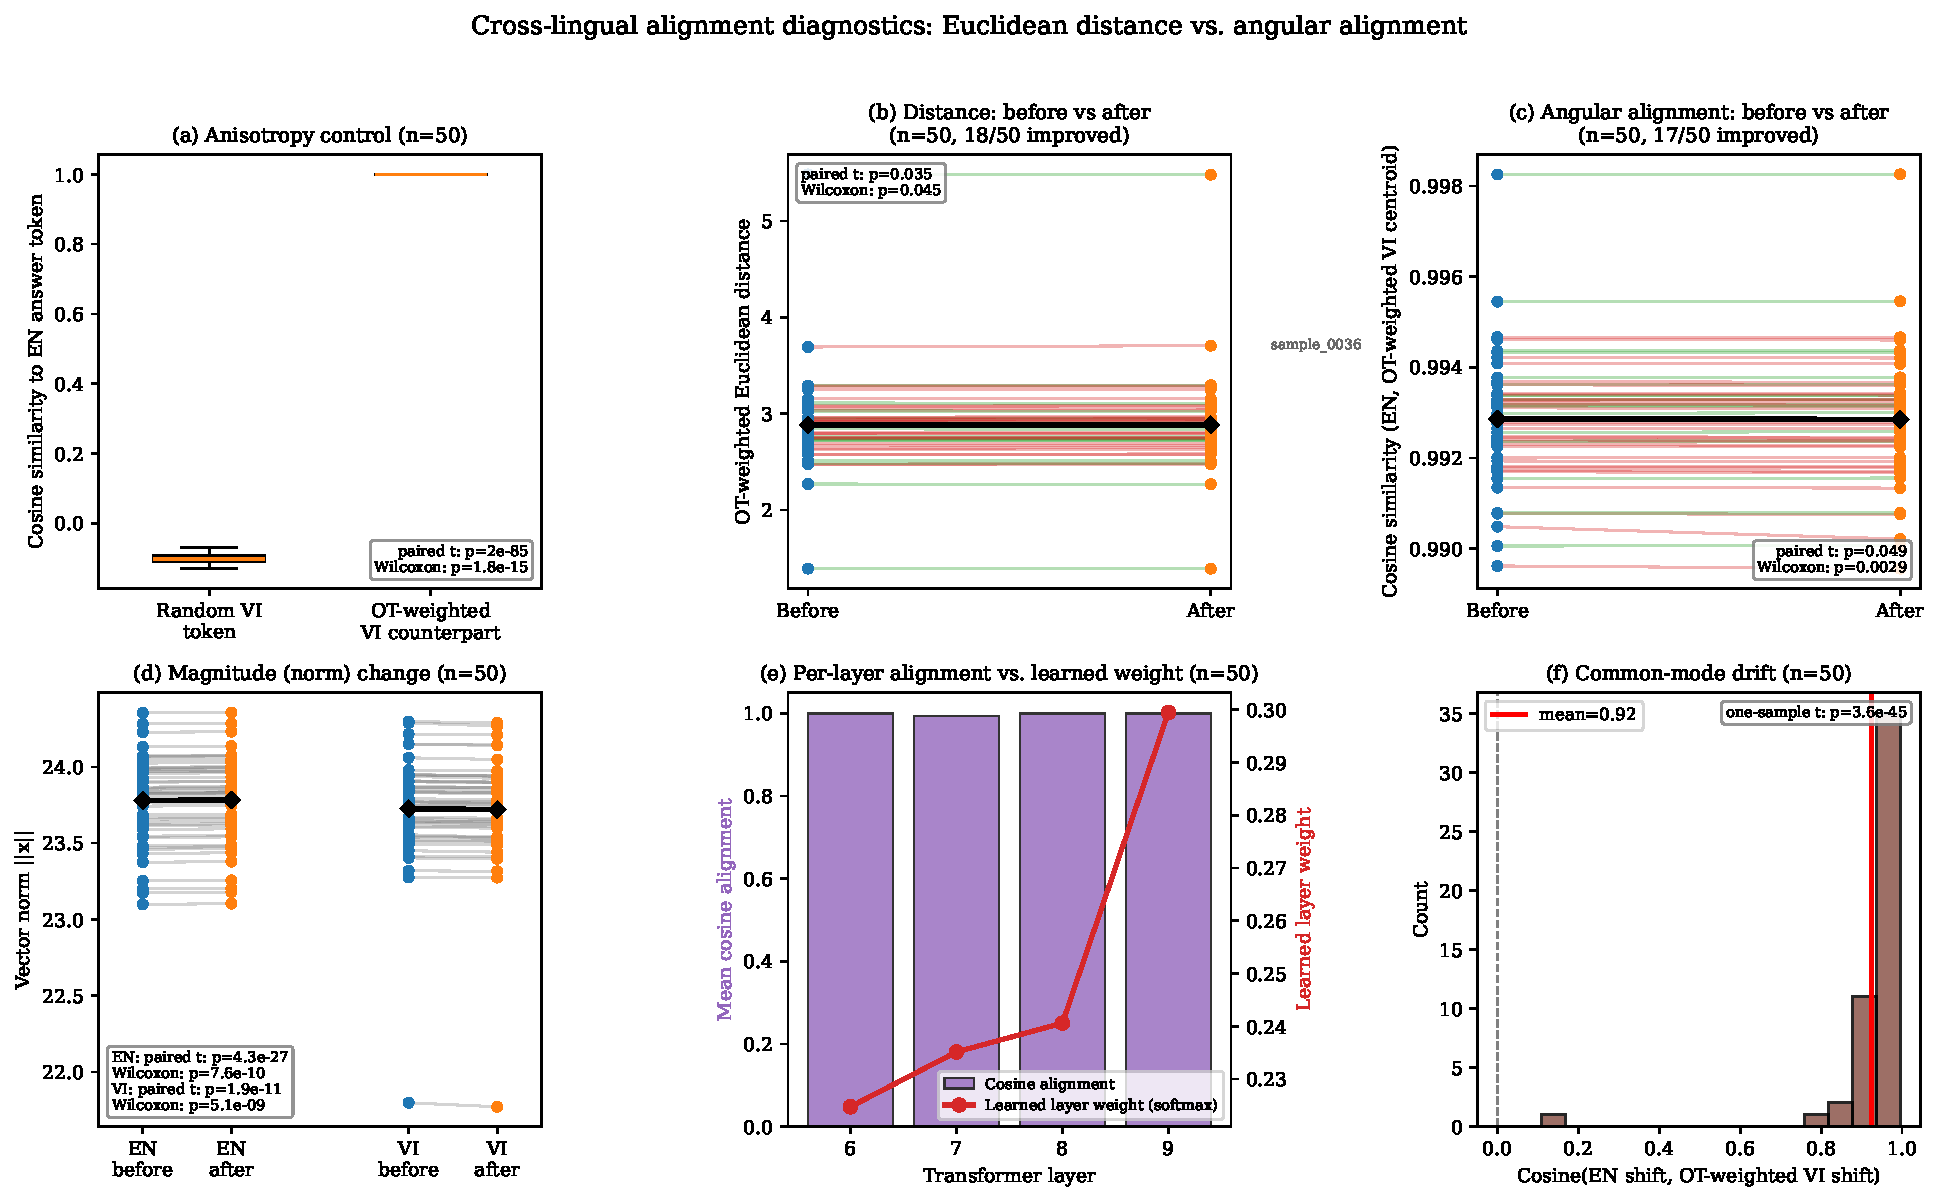
\includegraphics[width=1.05\textwidth]{figures/figure_alignment_summary.pdf}
    \caption{Geometric diagnostics of the OT-weighted cross-lingual alignment ($n=50$ sampled pairs). (a) Anisotropy control: the OT-weighted Vietnamese counterpart is far more similar to the English answer token than a randomly sampled Vietnamese token, ruling out a trivial anisotropy artifact. (b--c) Euclidean distance and angular (cosine) alignment between English and OT-weighted Vietnamese representations, before and after Stage-2 adaptation. (d) Change in representation norm for English and Vietnamese tokens. (e) Per-layer cosine alignment against the learned softmax layer weight (cf.\ Figure~\ref{fig:layer_weights}), showing that the layer receiving the highest learned weight (layer 9) also exhibits the strongest alignment. (f) Common-mode drift: cosine similarity between the English and OT-weighted Vietnamese shift vectors is consistently high (mean $=0.90$), indicating that adaptation moves both representations in a broadly coordinated direction.}
    \label{fig:alignment_diagnostics}
\end{figure*}

Figure~\ref{fig:alignment_diagnostics} summarizes these diagnostics, computed over $n=50$ sampled pairs. Panel (a) confirms that the OT-weighted correspondence is non-trivial: cosine similarity to the true English answer token is near $1.0$ for the OT-selected Vietnamese counterpart, against near-zero for a random Vietnamese token ($p=2.3\times10^{-81}$, paired $t$-test), ruling out a trivial anisotropy artifact.

Panel (b) shows that raw Euclidean distance between English and OT-weighted Vietnamese representations increases slightly but consistently after adaptation: 49 of 50 pairs show an increase, with a median shift of only $+0.005$ and a mean shift of $+0.015$ (paired $t$ $p=0.0023$, Wilcoxon $p=8\times10^{-10}$). Here it is the consistency of direction across nearly all pairs, rather than the magnitude of the shift -- under $1\%$ of the median pre-adaptation distance of $\approx 3.1$ -- that drives significance; a small number of pairs with much larger absolute distances (e.g., sample\_0044) inflate the mean without changing the qualitative pattern.

Panel (c) is more equivocal than panel (b), and we report this honestly rather than the more optimistic picture a smaller sample suggested. At $n=50$, the angular (cosine) alignment shift is \emph{not} statistically significant (paired $t$ $p=0.089$, Wilcoxon $p=0.15$): a bare majority of pairs (33/50) shift in the improving direction, but the median change is essentially zero ($+0.00001$) and the mean is pulled slightly negative by a handful of pairs with larger degradations. An earlier diagnostic on a smaller $n=20$ subset had suggested a clearer positive trend (18/20 improved, Wilcoxon $p=0.012$); this larger and more representative sample does not replicate that effect as statistically reliable, and we treat angular alignment as an open question for this framework rather than a confirmed improvement.

Panel (d) reports the accompanying change in representation norm for both languages ($n=50$), and deserves a direct comment given the role of $\mathcal{L}_{reg}$. Both English and Vietnamese tokens show a statistically significant shift in magnitude (English: paired $t$ $p=3.9\times10^{-76}$, Wilcoxon $p=7.6\times10^{-10}$; Vietnamese: paired $t$ $p=1.5\times10^{-6}$, Wilcoxon $p=2.4\times10^{-6}$), and the English shift is in fact associated with the smaller $p$-value of the two, despite English being the side explicitly anchored by $\mathcal{L}_{reg}$. Computing the underlying effect sizes resolves this: the mean English norm shift is $+0.066$ ($\mathrm{SD}=0.002$, a $0.28\%$ relative change, range $[0.062, 0.070]$ across the 50 pairs), whereas the mean Vietnamese shift is smaller in magnitude ($+0.049$, a $0.21\%$ relative change) but far more variable ($\mathrm{SD}=0.063$, range $[-0.246, 0.078]$). In other words, English does not shift more than Vietnamese in absolute terms -- if anything, slightly less -- but it shifts by an almost identical amount for every sampled pair, which is what drives its more extreme $p$-value under a paired test: statistical significance here reflects the \emph{consistency} of the shift's direction and magnitude across pairs, not its size. This pattern is consistent with the English shift being a small, systematic calibration effect induced uniformly by the LoRA adapters (largely input-independent to first order), rather than input-specific representation drift; the substantially larger and more dispersed Vietnamese shift, in contrast, reflects genuine per-example structural reorganization under the OT-guided pull toward the source space, exactly as the framework is designed to induce. Both shifts remain under $0.3\%$ of the total vector norm, supporting the ``soft anchor, not frozen'' interpretation of $\mathcal{L}_{reg}$ without requiring the encoder to be exactly invariant.

Panel (e) provides direct evidence for the layer-weighting behavior discussed above: alignment quality increases with depth across layers 6--9, mirroring the learned softmax weights. Finally, panel (f) shows that the direction of representation shift induced by adaptation remains highly correlated between languages even at $n=50$ (one-sample $t$-test, $p=7.1\times10^{-33}$, mean cosine $=0.90$), supporting the claim that our coordination mechanism moves source and target representations in a broadly coordinated direction rather than distorting their relative geometry arbitrarily.

\section{Hyperparameter Sensitivity and Loss Scale Normalization}
\label{sec:appendix_sensitivity}
The multi-objective parameters $\lambda_{ot}$, $\lambda_{span}$, $\lambda_{reg}$, and $\lambda_{margin}$ function as loss-scale normalizers to bring different objectives to a comparable magnitude. The source representation consistency coefficient ($\lambda_{reg}$) dominates with a value of $50.0$, which is structurally required because the native token-level $L_2$ deviation scales within a significantly smaller numerical range ($0.008$ to $0.01$). 

We performed a grid search variation over $\lambda_{reg} \in \{0.0, 10.0, 50.0, 100.0\}$. Setting $\lambda_{reg} < 10.0$ induces a severe representation drift in the shared LoRA blocks, resulting in an immediate collapse of English QA proficiency. Conversely, setting $\lambda_{reg} > 100.0$ over-regularizes the adapter weights, restricting the student's capacity to adjust its latent representations to the target language topology.

\section{Optimization Dynamics: Curriculum vs. Static Margin}
\label{sec:appendix_margin_dynamics}
The full training trajectories comparing the static decision-boundary margin (configuration M4) against our dynamic curriculum margin schedule (configuration M5), along with the accompanying trade-off discussion, are presented in Section~\ref{sec:margin_impact} and Figures~\ref{fig:margin_dynamics_xquad}--\ref{fig:margin_dynamics_mlqa} to avoid duplicating the same figures here.

\section{Qualitative Case Study: Visualizing Answer Span Boundaries}
\label{sec:appendix_case_study}
To qualitatively demonstrate how our coordinated framework prevents answer-boundary ambiguity, we extract a translation-shifted paragraph sample from the evaluation benchmark. 
\begin{figure}[H]
    \centering
    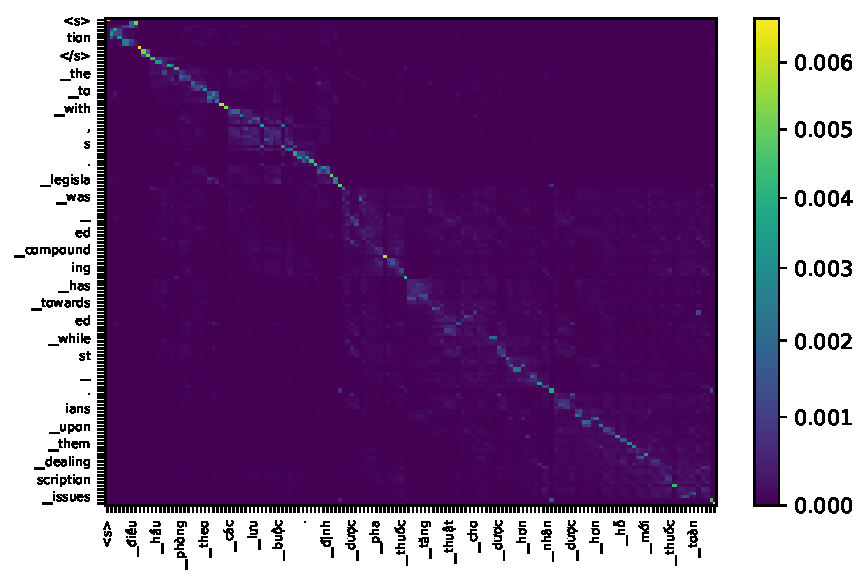
\includegraphics[width=1.05\linewidth]{figures/figure2_ot_heatmap.pdf}
    \caption{Visualization of the log-domain Sinkhorn transport plan ($\gamma$) aligning source English tokens (rows) with target Vietnamese tokens (columns) for a representative XQuAD-vi example. Transport mass concentrates near the diagonal with a few coherent off-diagonal bands, indicating that the plan recovers meaningful token-level correspondence despite word-segmentation and word-order differences between the two languages.}
    \label{fig:case_study}
\end{figure}

The transport plan visualization in Figure \ref{fig:case_study} shows that alignment mass is concentrated in coherent, low-noise bands rather than being diffusely spread across unrelated tokens, consistent with our claim that the OT plan produces a structurally meaningful cross-lingual correspondence. This qualitative pattern is consistent with the quantitative margin behavior in Table~\ref{tab:ablation_study}: because the Curriculum Margin keeps the top-1/top-2 task-space logit gap discriminative throughout training, the resulting transport-guided pseudo-labels translate into coherent rather than diffuse predicted spans. A side-by-side visualization of predicted spans under the static versus dynamic margin schedule on this same example is left for future work.
\end{document}